\documentclass[tikz,border=3pt]{standalone}
\usetikzlibrary{arrows.meta,calc}
\begin{document}
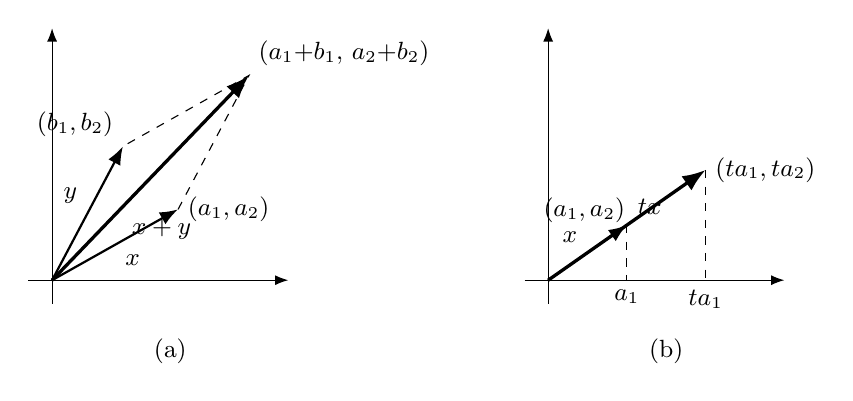
\begin{tikzpicture}[>=Latex, font=\small]
  % --- panel izquierdo: suma en coordenadas ---
  \begin{scope}
    \coordinate (O) at (0,0);
    \coordinate (X) at (1.6,0.9);
    \coordinate (Y) at (0.9,1.7);
    \coordinate (Q) at ($(X)+(Y)$);

    \draw[->] (-0.3,0) -- (3.0,0);
    \draw[->] (0,-0.3) -- (0,3.2);

    \draw[dashed] (X) -- (Q) -- (Y);
    \draw[->, thick] (O) -- (X) node[midway, below right] {$x$};
    \draw[->, thick] (O) -- (Y) node[midway, above left] {$y$};
    \draw[->, very thick] (O) -- (Q) node[pos=0.35, below right] {$x+y$};

    \node[right] at (X) {$(a_1,a_2)$};
    \node[above left] at (Y) {$(b_1,b_2)$};
    \node[above right] at (Q) {$(a_1{+}b_1,\,a_2{+}b_2)$};
    \node at (1.5,-0.9) {(a)};
  \end{scope}

  % --- panel derecho: multiplicacion escalar ---
  \begin{scope}[shift={(6.3,0)}]
    \coordinate (O) at (0,0);
    \coordinate (X) at (1.0,0.7);
    \coordinate (TX) at (2.0,1.4);

    \draw[->] (-0.3,0) -- (3.0,0);
    \draw[->] (0,-0.3) -- (0,3.2);

    \draw[->, very thick] (O) -- (TX) node[midway, above right] {$tx$};
    \draw[->, thick] (O) -- (X) node[midway, above left] {$x$};

    \draw[dashed] (X) -- (1.0,0);
    \draw[dashed] (TX) -- (2.0,0);
    \node[below] at (1.0,0) {$a_1$};
    \node[below] at (2.0,0) {$ta_1$};
    \node[right] at (TX) {$(ta_1,ta_2)$};
    \node[above left=-1mm] at (X) {$(a_1,a_2)$};
    \node at (1.5,-0.9) {(b)};
  \end{scope}
\end{tikzpicture}
\end{document}
